\section{Architettura}
\subsection{Pattern architetturale: MVC}
\begin{figure}[H]
    \centering
    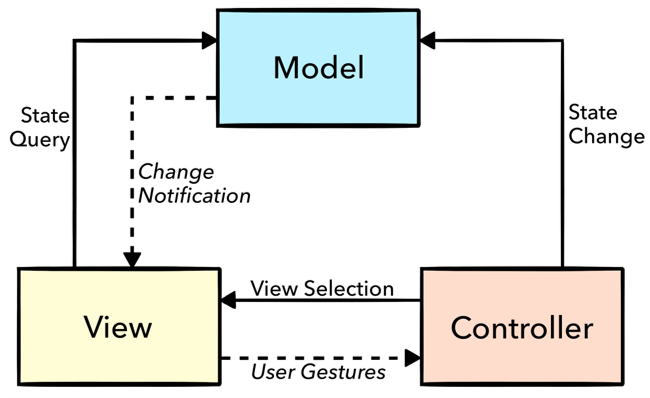
\includegraphics[scale = 1]{components/img/mvc-generico.png}
    \caption{Diagramma pattern MVC}
    \label{fig:diagramma MVC generico}
\end{figure}
L'architettura del capitolato C7 aderisce al pattern architetturale \textit{Model-View-Controller (MVC).} L'aderenza al pattern era un requisito obbligatorio imposto dall'azienda ma sono stati riscontrati diversi punti positivi nella sua implementazione:

\begin{itemize}
    \item Rapidità nello sviluppo software dato dalla possibilità di lavoro parallelo su modello, vista e controller;
    \item Indipendenza dei vari componenti;
    \item Maggior facilità nella testabilità, manutenibilità e scalabilità.
\end{itemize}

\subsection{Diagramma dei pacchetti}
\begin{figure}[H]
    \centering
    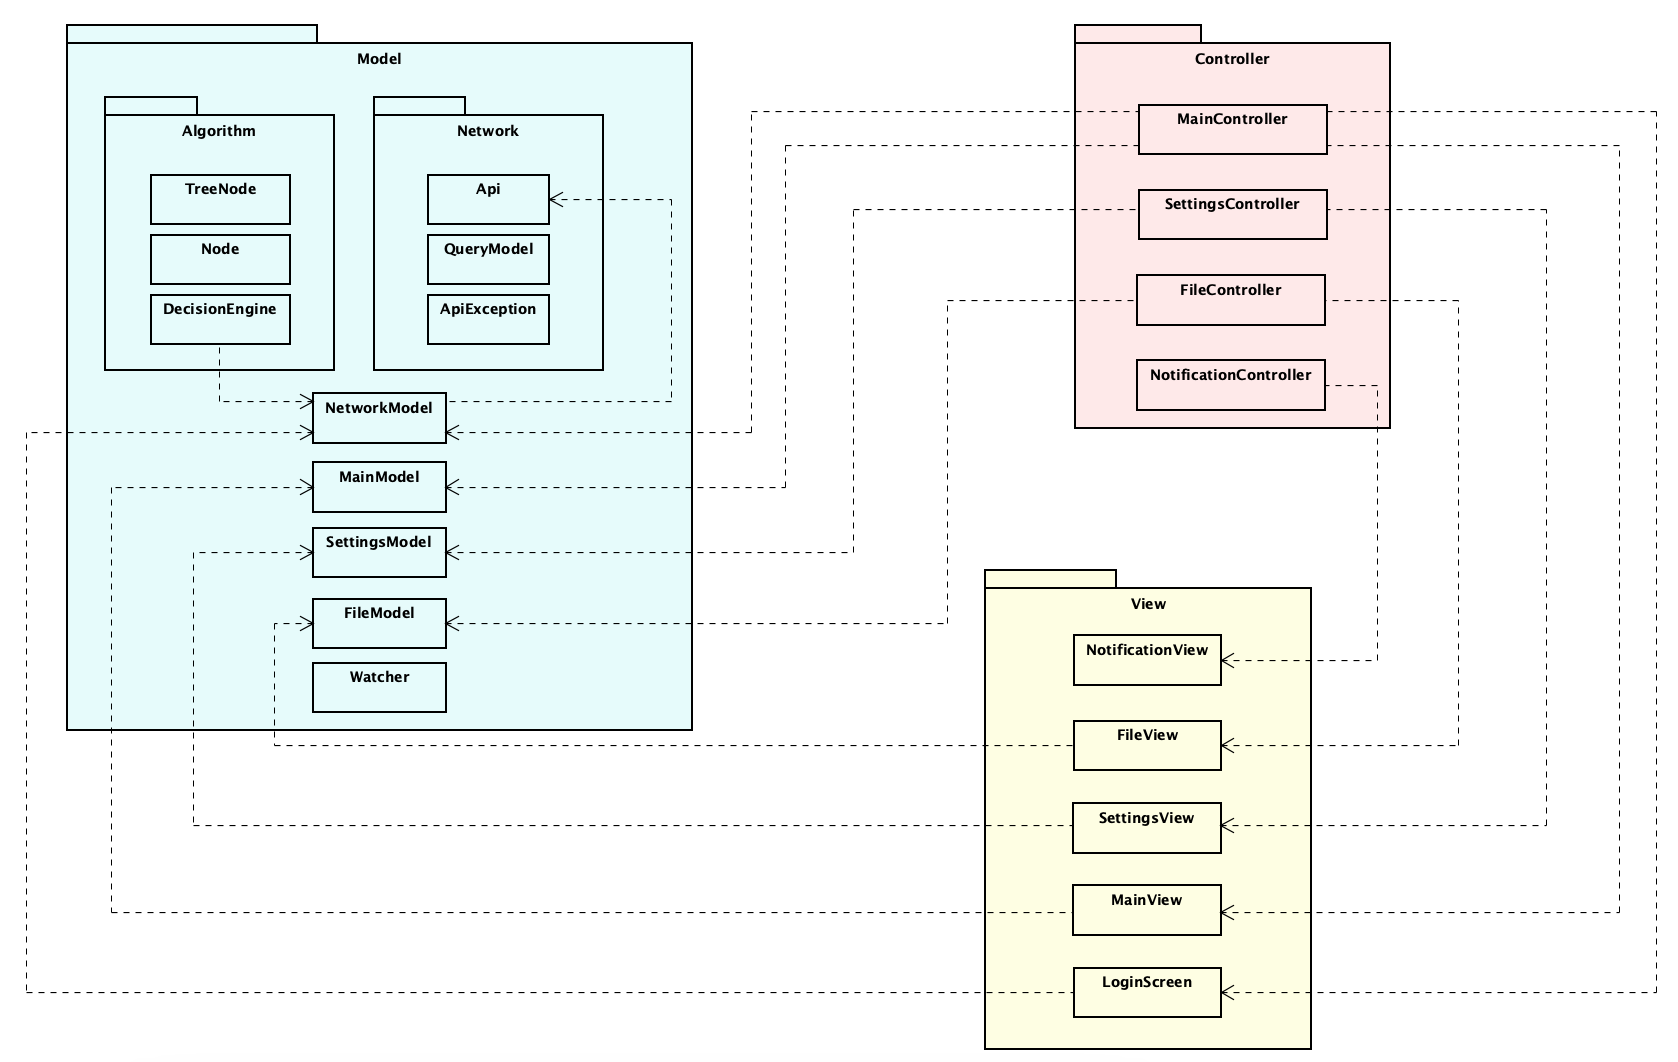
\includegraphics[scale = 0.5]{components/img/diagramma-package.png}
    \caption{Diagramma pacchetti}
    \label{fig:diagramma pacchetti}
\end{figure}
\subsection{Diagramma delle classi - model}

\begin{figure}[H]
    \centering
    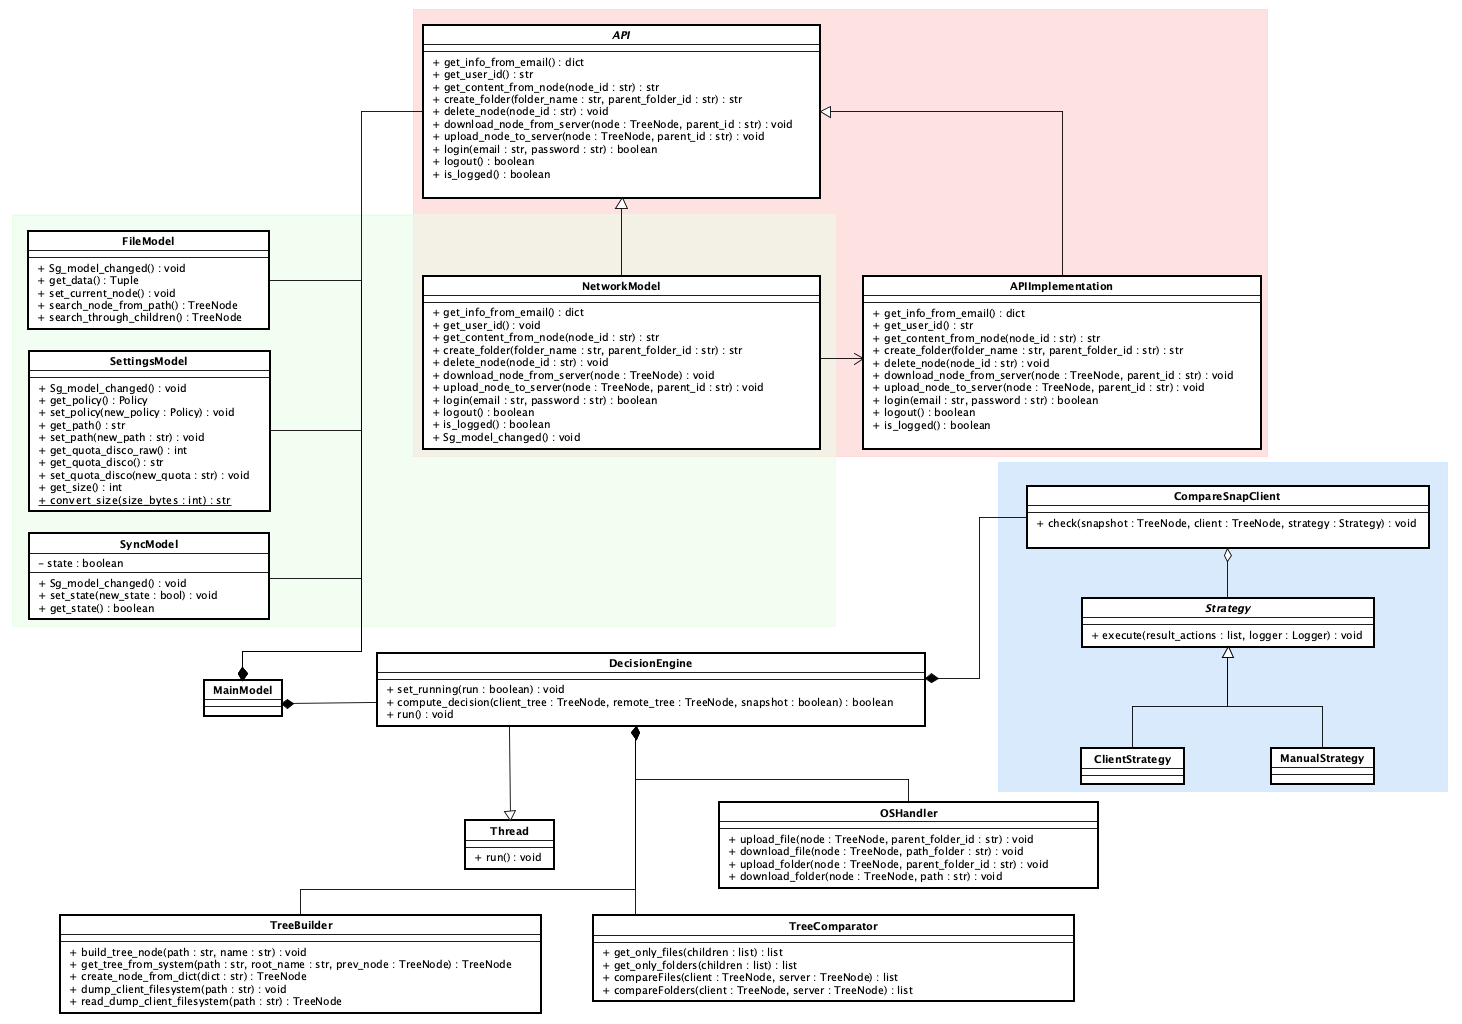
\includegraphics[scale = 0.6]{components/img/diagramma-classi-model.png}
    \caption{Diagramma delle classi nel model}
    \label{fig:Diagramma delle classi nel model}
\end{figure}

\subsection{Design pattern creazionali: Singleton}

Le classi mostrate in figura 3 rispettano il pattern singleton, il che le porta ad avere una sola loro istanza all'interno del programma.
\newline{}
L'implementazione del pattern in Python è stata possibile grazie alla funzione get\_instance, presente in ogni classe,  che controlla se essa è stata istanziata o meno. In caso negativo crea la nuova istanza e, nelle chiamate successive, si limita a restituire la stessa. Il costruttore della classe, quindi, può essere chiamato solamente all'interno di get\_instance. \newline{}
Il pattern singleton può provocare problemi se mal implementato. Nel nostro caso, l'implementazione è corretta in quanto l'istanza dei vari modelli è passata ai costruttori di tutti gli utilizzatori. Questo permette la realizzazione degli unit test che, altrimenti, sarebbero impossibili da implementare. 
\begin{figure}[H]
    \centering
    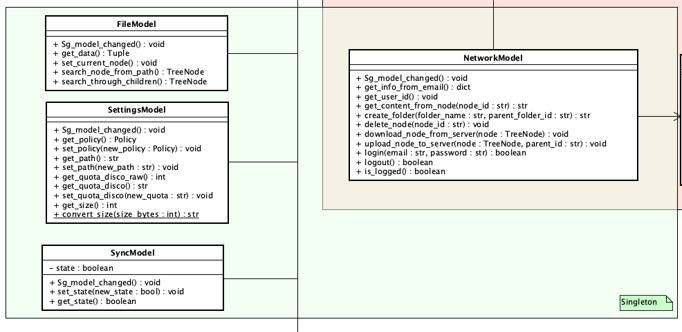
\includegraphics[scale = 0.43]{components/img/singleton-model.png}
    \caption{Pattern Singleton nel dettaglio}
    \label{fig:Diagramma del pattern singleton}
\end{figure}
\subsection{Design pattern strutturali: Virtual Proxy}
Il pattern Proxy viene utilizzato per evitare chiamate di rete non necessarie, permettendo la lazy initialization.\newline{}
Questo pattern in Python è stato realizzato tramite il modulo ABC (Abstract Base Classes) realizzando la classe astratta API che viene ereditata da NetworkModel e da APIImplementation. In questo modo si vanno a definire dei metodi base che entrambe le classi condividono. Quando verrà effettuata una chiamata di rete si passa per NetworkModel che, dopo controlli aggiuntivi, potrà decidere se passare la chiamata ad APIImplementation. Facendo riferimento al modello del pattern, NetworkModel è il nostro proxy e APIImplementation il nostro realsubject.
\begin{figure}[H]
    \centering
    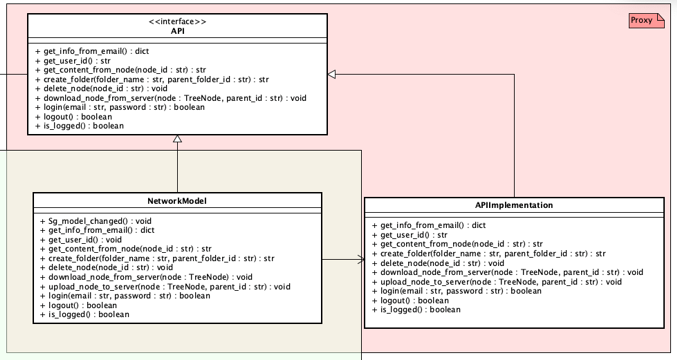
\includegraphics[scale = 0.45]{components/img/proxy-model.png}
    \caption{Pattern Proxy nel dettaglio}
    \label{fig:Pattern proxy nel dettaglio}
\end{figure}
\subsection{Design pattern comportamentali:}
\subsubsection{Observer:}
Il patter observer è stato implementato usando i segnali e slot forniti dalla libreria PySide6, vengono usati per la communicazione tra diversi oggetti.
Segnali e slot vengono usati per le communicazioni fra model, controller e view. I segnali emessi dal model e dalla view vengono usati dalla classe Signal che chiamerà gli slot collegati ad essi. La classe view e controller ereditano dall'interfaccia Slot.
\begin{figure}[H]
    \centering
    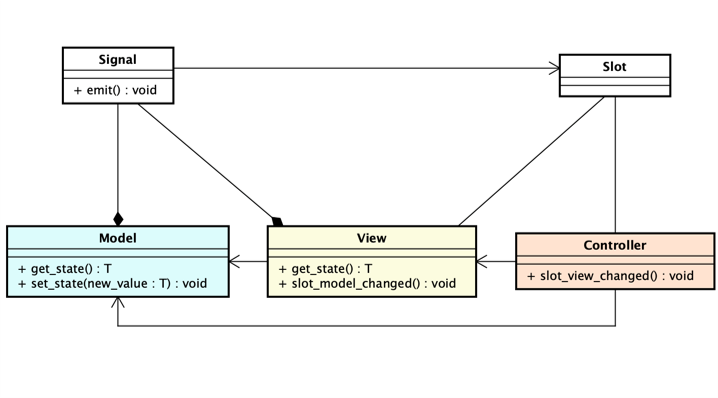
\includegraphics[scale = 0.45]{components/img/observer-implementazione.png}
    \caption{Pattern Observer con segnali e slot nel dettaglio}
    \label{fig:Pattern observer con segnali e slot}
\end{figure}

\subsubsection{Strategy:}
La scelta di utilizzare questo pattern è stata naturale poiché esso va a descrivere pienamente la realtà del \textit{capitolato C7}.\newline{}
Attualmente si hanno due diverse politiche per la sincronizzazione che posso essere scelte a runtime e che variano il comportamento dell'algoritmo. Si ha una classe CompareSnapClient che fa da interfaccia comune e chiama al suo interno il metodo execute della classe attualmente scelta. Essendo Strategy una classe astratta, essa fornisce il metodo execute che deve essere implementato da tutte le classi figlie. Questo permette all' istanza di CompareSnapClient di poter chiamare il metodo execute di un qualsiasi oggetto Strategy di cui non conosce l'implementazione. L'adozione del suddetto pattern permette l'aggiunta di nuove politiche senza dover cambiare la logica dell'applicazione, il che semplificherà il lavoro in eventuali sviluppi futuri.

\begin{figure}[H]
    \centering
    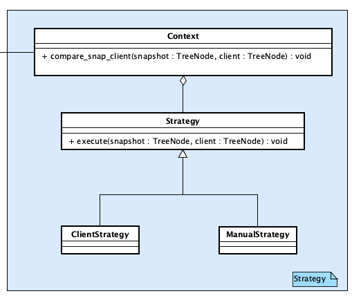
\includegraphics[scale = 0.45]{components/img/strategy-model.png}
    \caption{Pattern Strategy nel dettaglio}
    \label{fig:Pattern proxy nel dettaglio}
\end{figure}
